
\documentclass[12pt]{article}

\usepackage[T1]{fontenc}
\usepackage[utf8]{inputenc}
\usepackage[french]{babel}
\usepackage{amsmath}
\usepackage{amssymb}
\usepackage[top=1.5cm, bottom=1.5cm, left=1.5cm, right=1.5cm]{geometry}
\usepackage{graphicx}
\usepackage{multicol}
\usepackage{lipsum}
\usepackage{eurosym}
\usepackage{indentfirst}
\usepackage{titlesec}
\usepackage{pifont}
\usepackage{url}
\usepackage{epsf}
\usepackage{listings}
\newcommand\tab[1][1cm]{\hspace*{#1}}
\begin{document}
    \begin{titlepage}
        \newcommand{\HRule}{\rule{\linewidth}{0.5mm}}
        \center
        \textsc{\LARGE
        UNIVERSITE CAEN-NORMANDIE
        } \\[1cm]
        
\includegraphics[scale=1]{images/LOGO-UNICAEN_V-2.2-N} \\[1cm]
        \HRule \\[0.4cm]
        { \huge \bfseries Rapport de développement: EASYTASK\\[0.15cm] }
        \HRule \\[1.5cm]
        KITSOUKOU Manne Emile\\[1cm]
        ALSEINY
        \\[1cm]
        \textbf{Licence 3 Informatique}\\
        \today \\ [1cm]
    \end{titlepage}
    \newpage
    \tableofcontents
    \newpage
    \section{Introduction}{\label{sec:intro}}

        Dans le cadre de la validation de l'UE( Unité d'Enseignement) de \textbf{Développement d'application web client},
        nous avons été amenés à réaliser une application de gestions de tâches. L'objectif de ce projet était de mettre
        en place une interface utilisateur intuitive, fonctionnel et ergonomique permettant à un utilisateur de gérer
        ses listes de tâches de maniere simple et efficace.\\

        Ce projet nous a permis de découvrir le framework \textbf{React native } tout en mettant en pratique nos
        connaissances en développement d'application mobiles. Nous avons dû faire face à des défis liés à la prise
        en main de ce nouvel outil, mais avons réussi à mettre en place une application fonctionnelle et ergonomique
        respectant les exigences de l'énoncé du projet. Cela a été également l'occassion de mettre en pratique nos
        connaissances des bases de données non traditionnelles à travers la mise en place d'une base de données
        \textbf{NoSQL} \textbf{GRAPHQL} à travers le service \textbf{Apollo NEO4J}.

        \section{Présentation de l'application}{\label{sec:app}}
        EASYTASK est une application de gestion de tâches. Elle permet à un utilisateur de créer des listes de tâches
        et de les gérer. Le développement à travers le framework \textbf{React native} permet de pouvoir utiliser
        l'application sur la plateformes \textbf{Android}, \textbf{IOS} et \textbf{Web}. Cela permet de rendre l'application
        plus accessible au plus grand nombre d'utilisateurs.\\
        L'application est divisée en différents écrans. Cette séparation permet de rendre l'application plus
        ergonomique et intuitive. L'utilisateur peut naviguer entre les différents écrans à travers des boutons
        présents sur chaque écran.\\

        \subsection{Ecrans d'authentification}{\label{subsec:auth}}
        L'application nécessite une authentification pour pouvoir accéder aux fonctionnalités de l'application.
        L'utilisateur doit donc se connecter à l'application à travers un formulaire d'authentification.\\
        \begin{figure}[H]
            \centering
            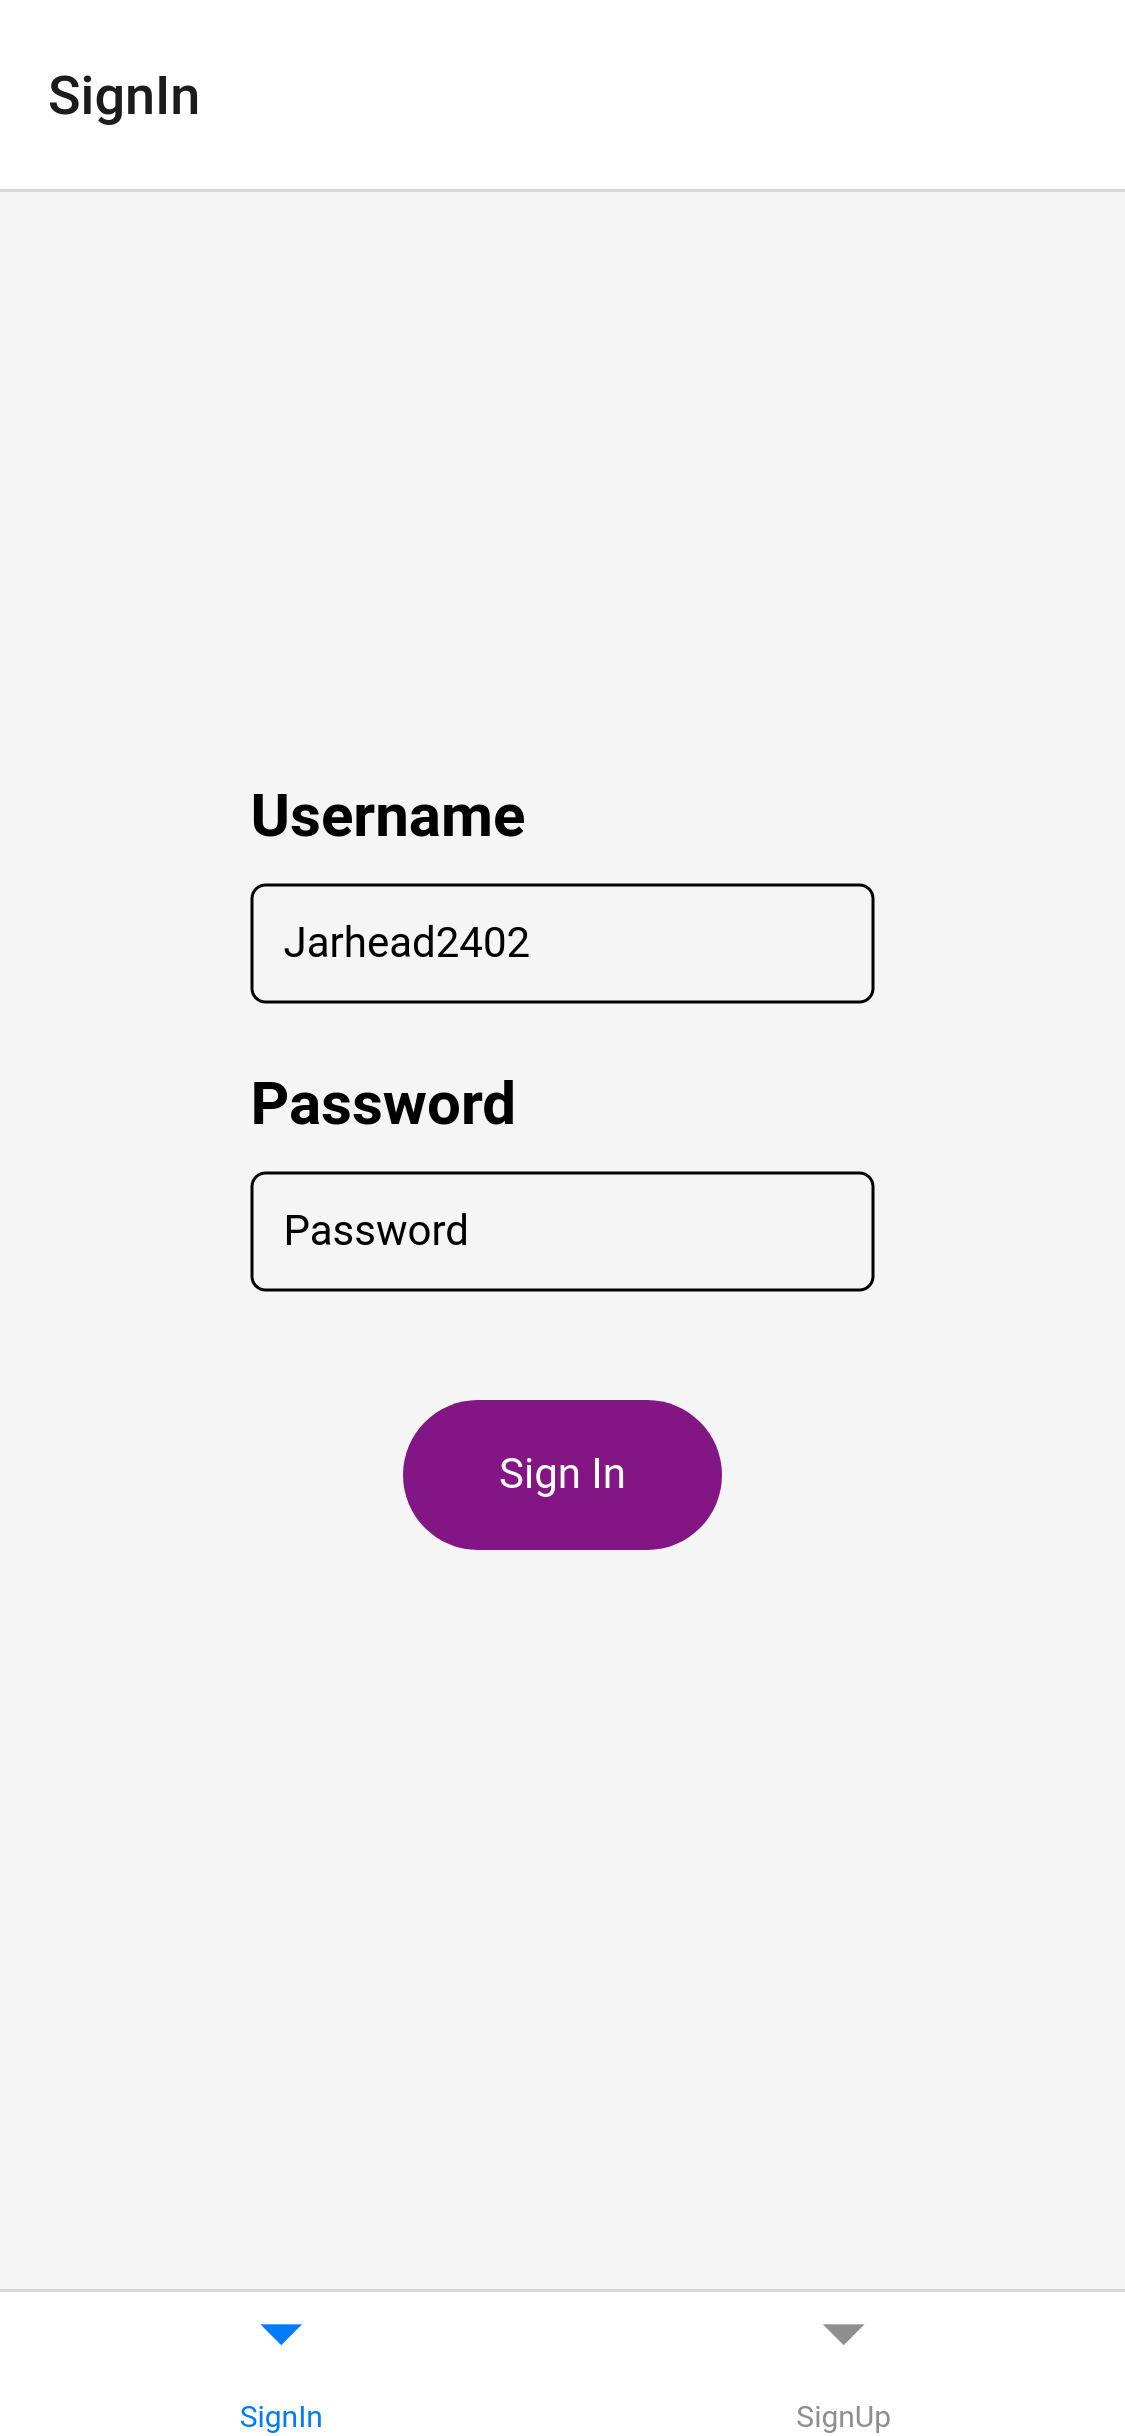
\includegraphics[width=0.4\textwidth]{images/signIn}
            \caption{Ecran d'authentification}
            \label{fig:auth}
        \end{figure}
        L'utilisateur doit renseigner son nom d'utilisateur et son mot de passe pour pouvoir accéder à l'application.
        Si l'utilisateur n'a pas de compte, il peut s'inscrire en cliquant sur le bouton \textbf{S'inscrire} présent
        en bas de l'écran.\\
        \begin{figure}[H]
            \centering
            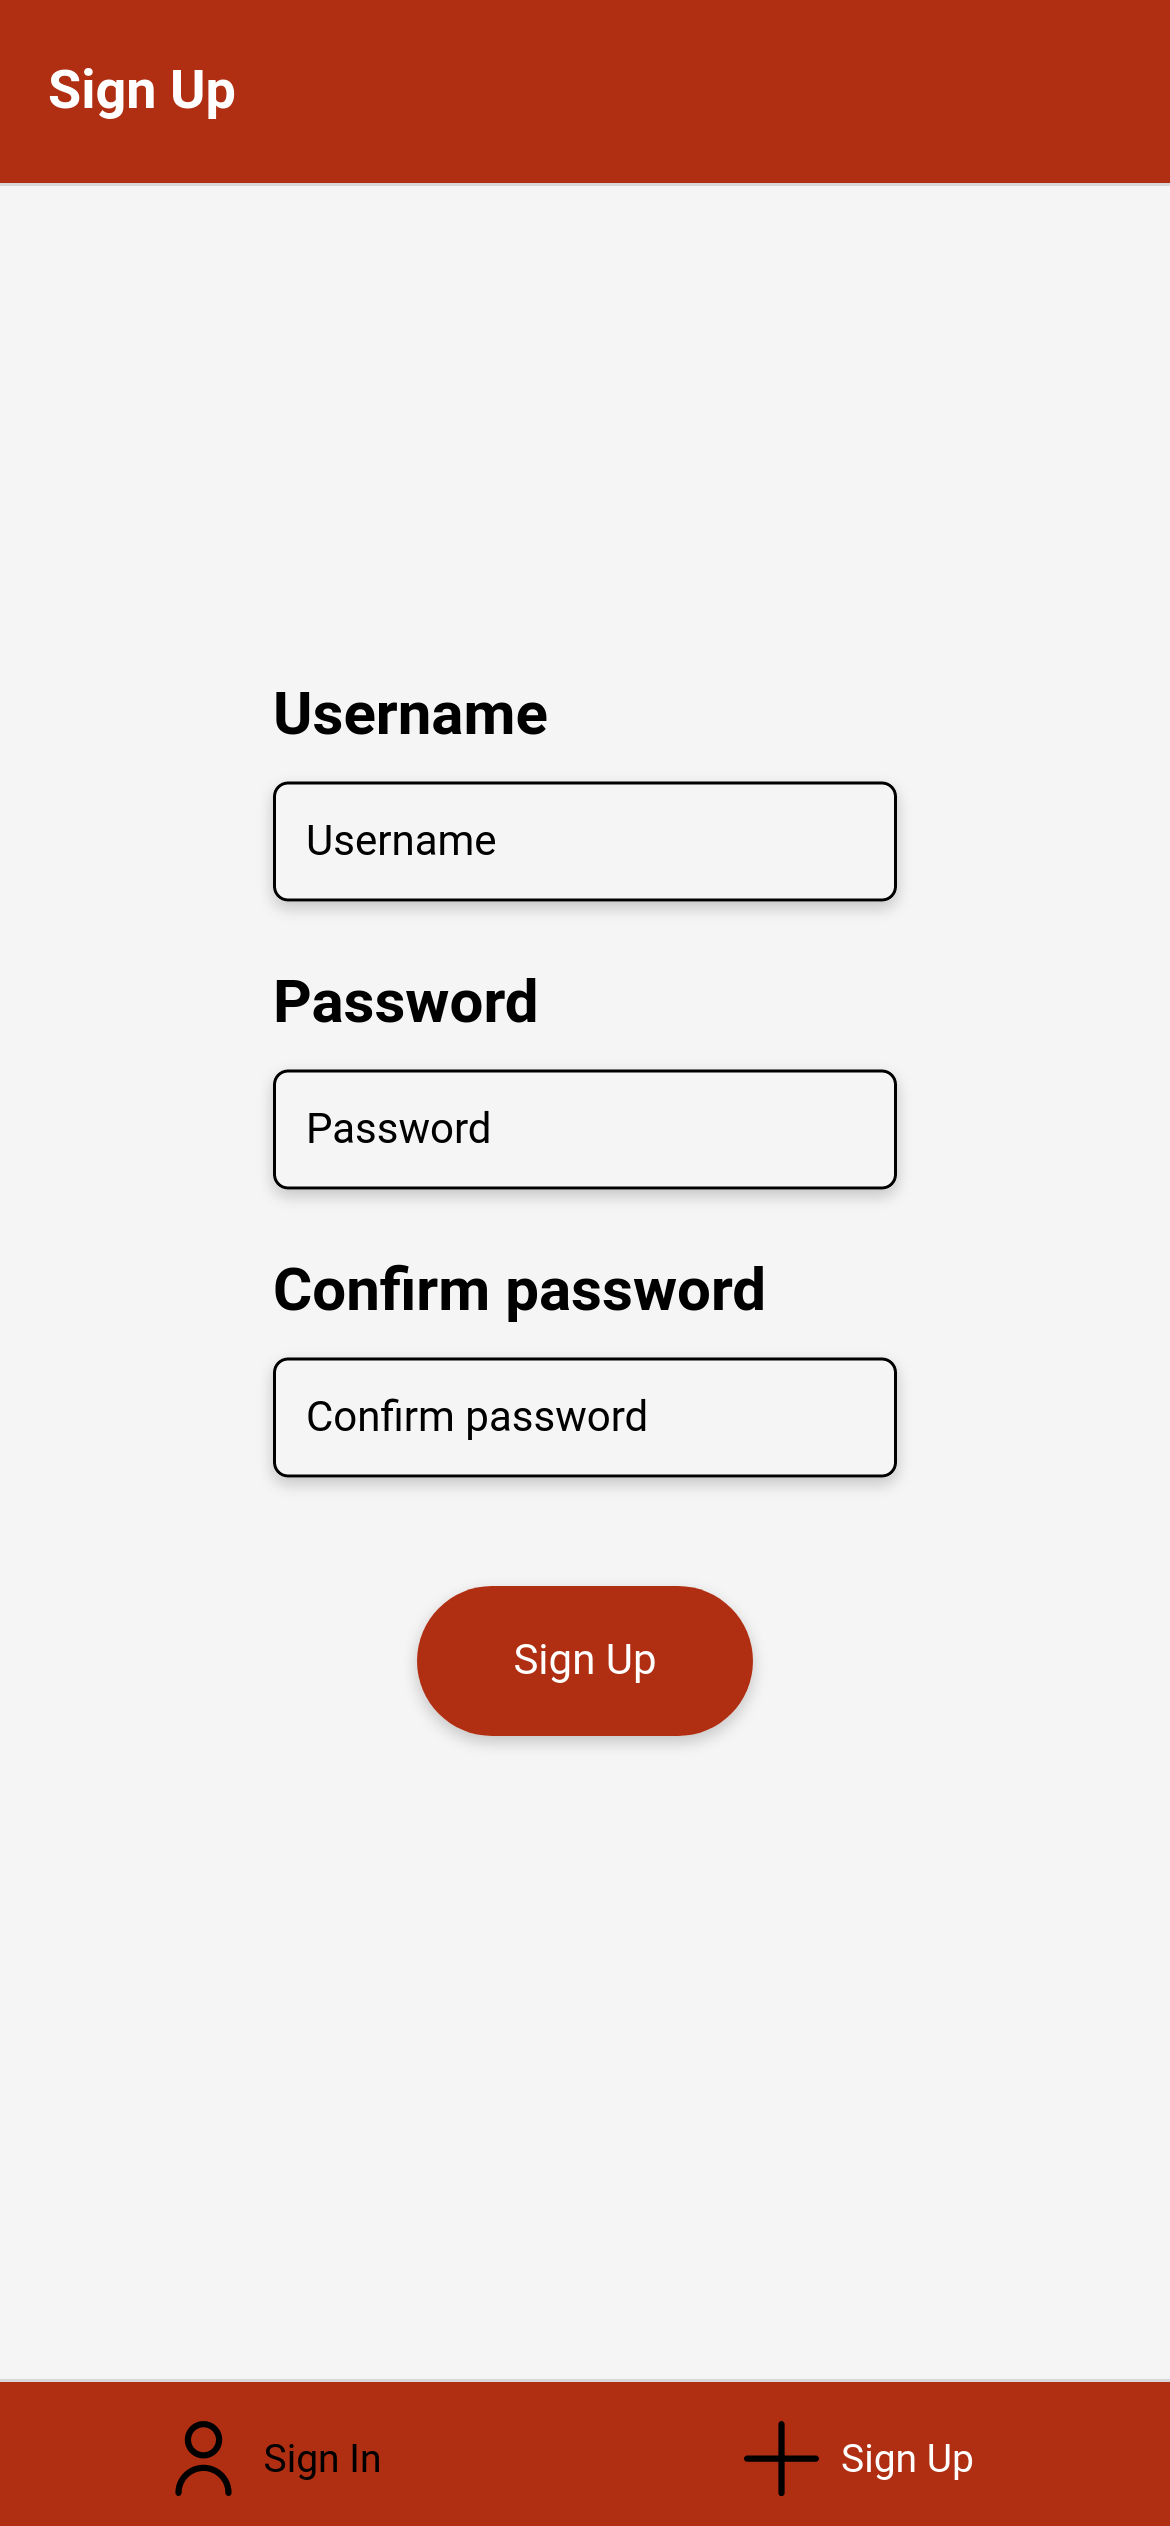
\includegraphics[width=0.4\textwidth]{images/signUp}
            \caption{Ecran d'inscription}
            \label{fig:insc}
        \end{figure}
        L'utilisateur doit renseigner son nom d'utilisateur, son mot de passe et sa confirmation.\\

        Cependant il faut noter que la réalisation de l'authentification reste basique.

        \subsection{Ecrans de gestion des listes de tâches}{\label{subsec:task}}
        Nous utilisons 2 ecrans pour gérer les listes de tâches. En effet, nous donnons la possibilités à l'utilisateurs
        de pouvoir manipuler plusieurs listes de taches. De ce fait, nous devrions avoir un écran principales qui permet
        d'afficher l'ensemble des listes de taches.
        \begin{figure}[H]
            \centering
            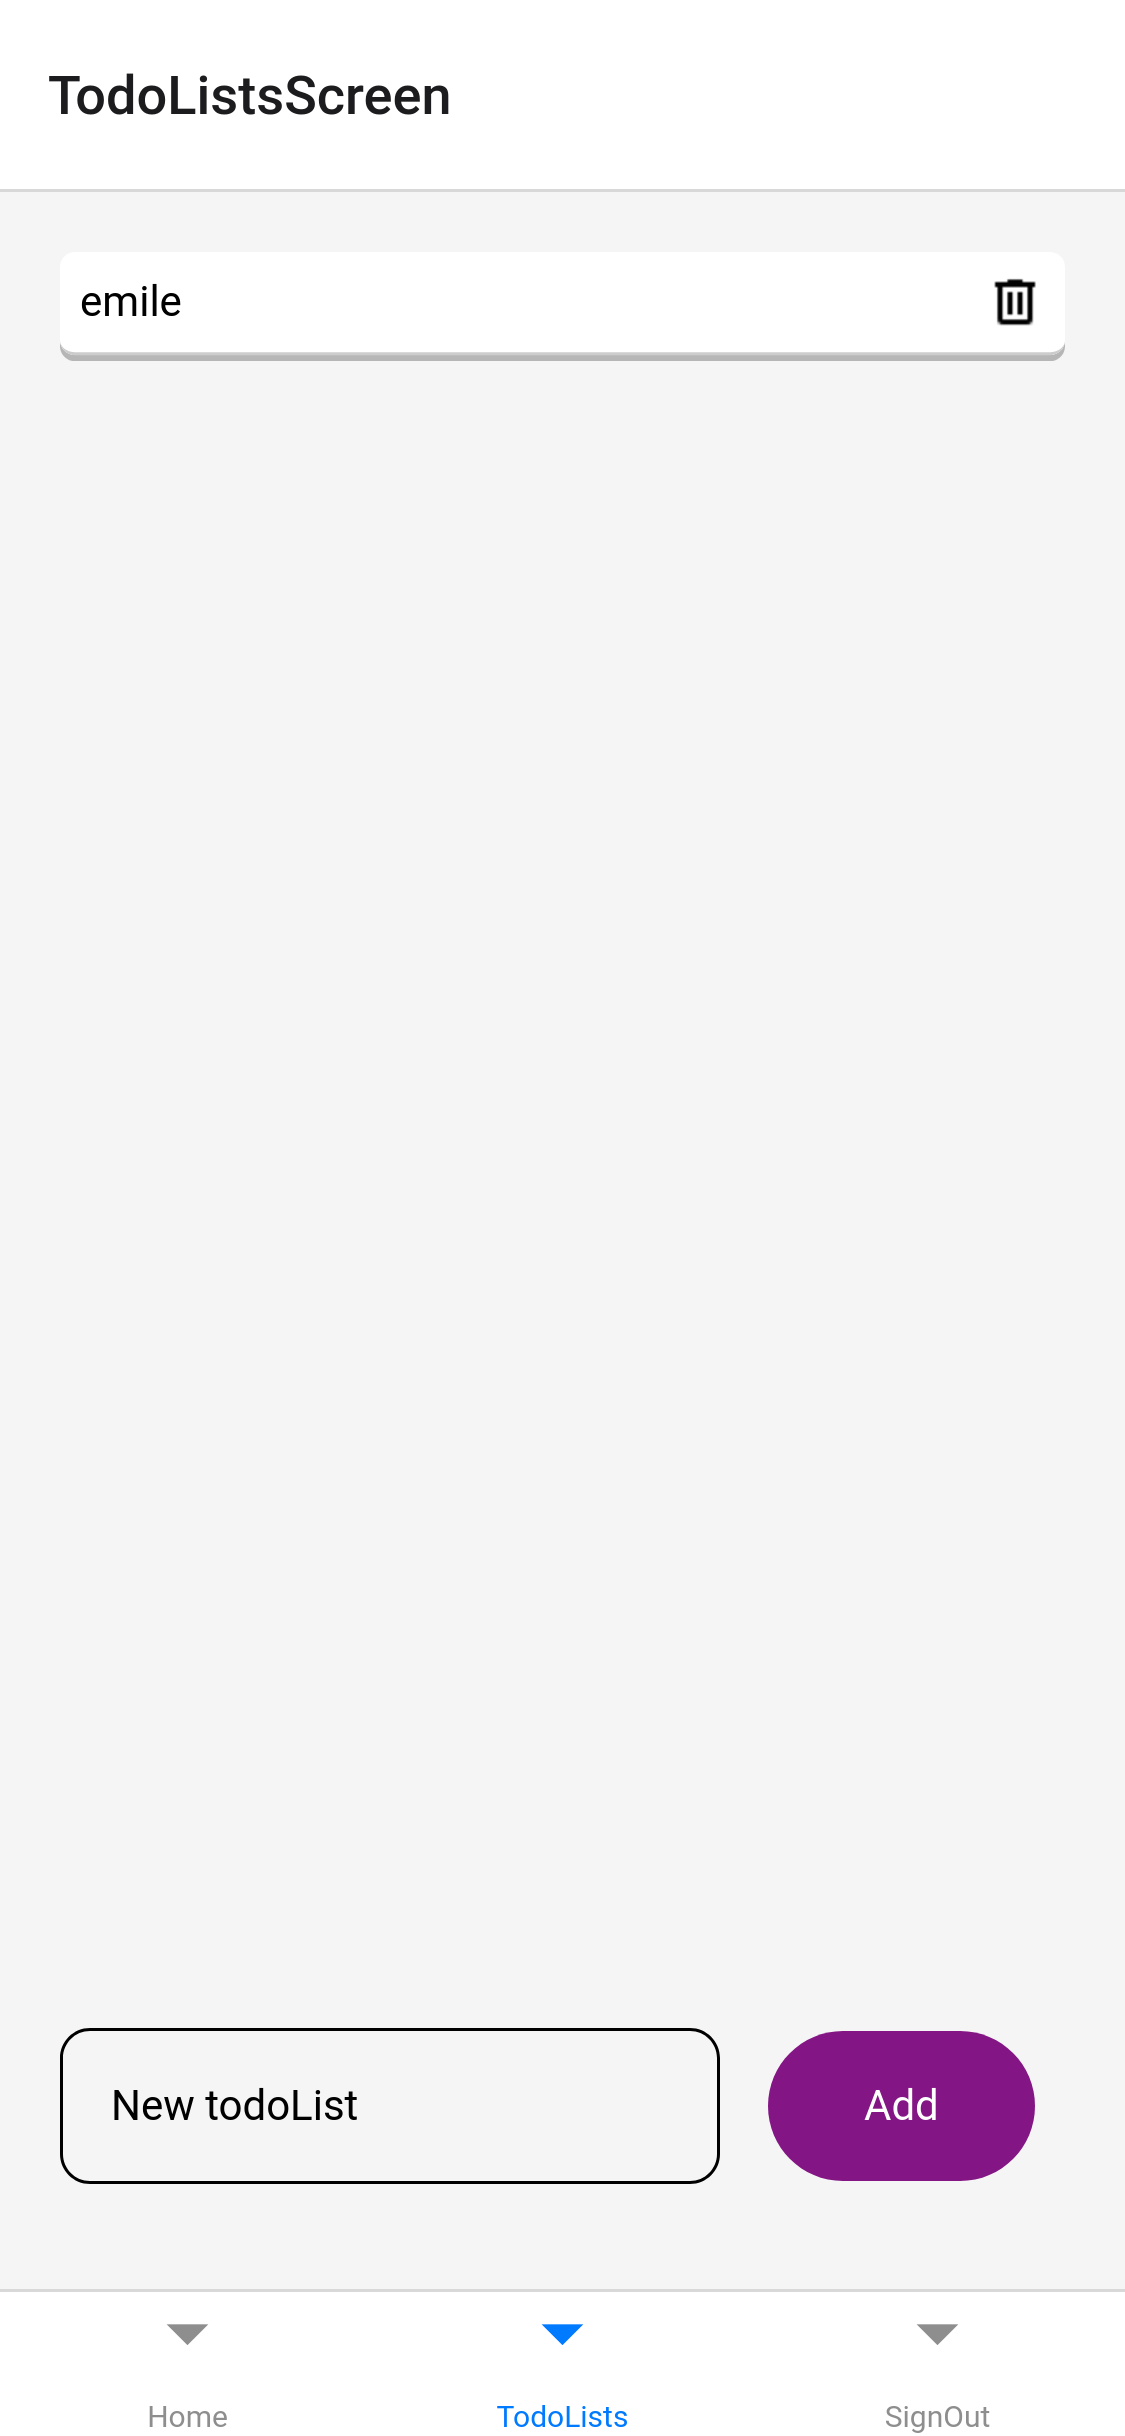
\includegraphics[width=0.2\textwidth]{images/taskList}
            \caption{Ecran de gestion des listes de tâches}
            \label{fig:taskList}
        \end{figure}
        L'utilisateur peut créer une nouvelle liste de tâches en cliquant sur le bouton \textbf{Nouvelle liste} présent
        après avoir renseigné le nom de la liste. Il peut également supprimer une liste de tâches en cliquant sur la poubelle
        présente à droite de chaque liste.\\
        En cliquant sur une liste de tâches, l'utilisateur est redirigé vers un écran qui lui permet de gérer les tâches
        de la liste.\\
        \begin{figure}[H]
            \centering
            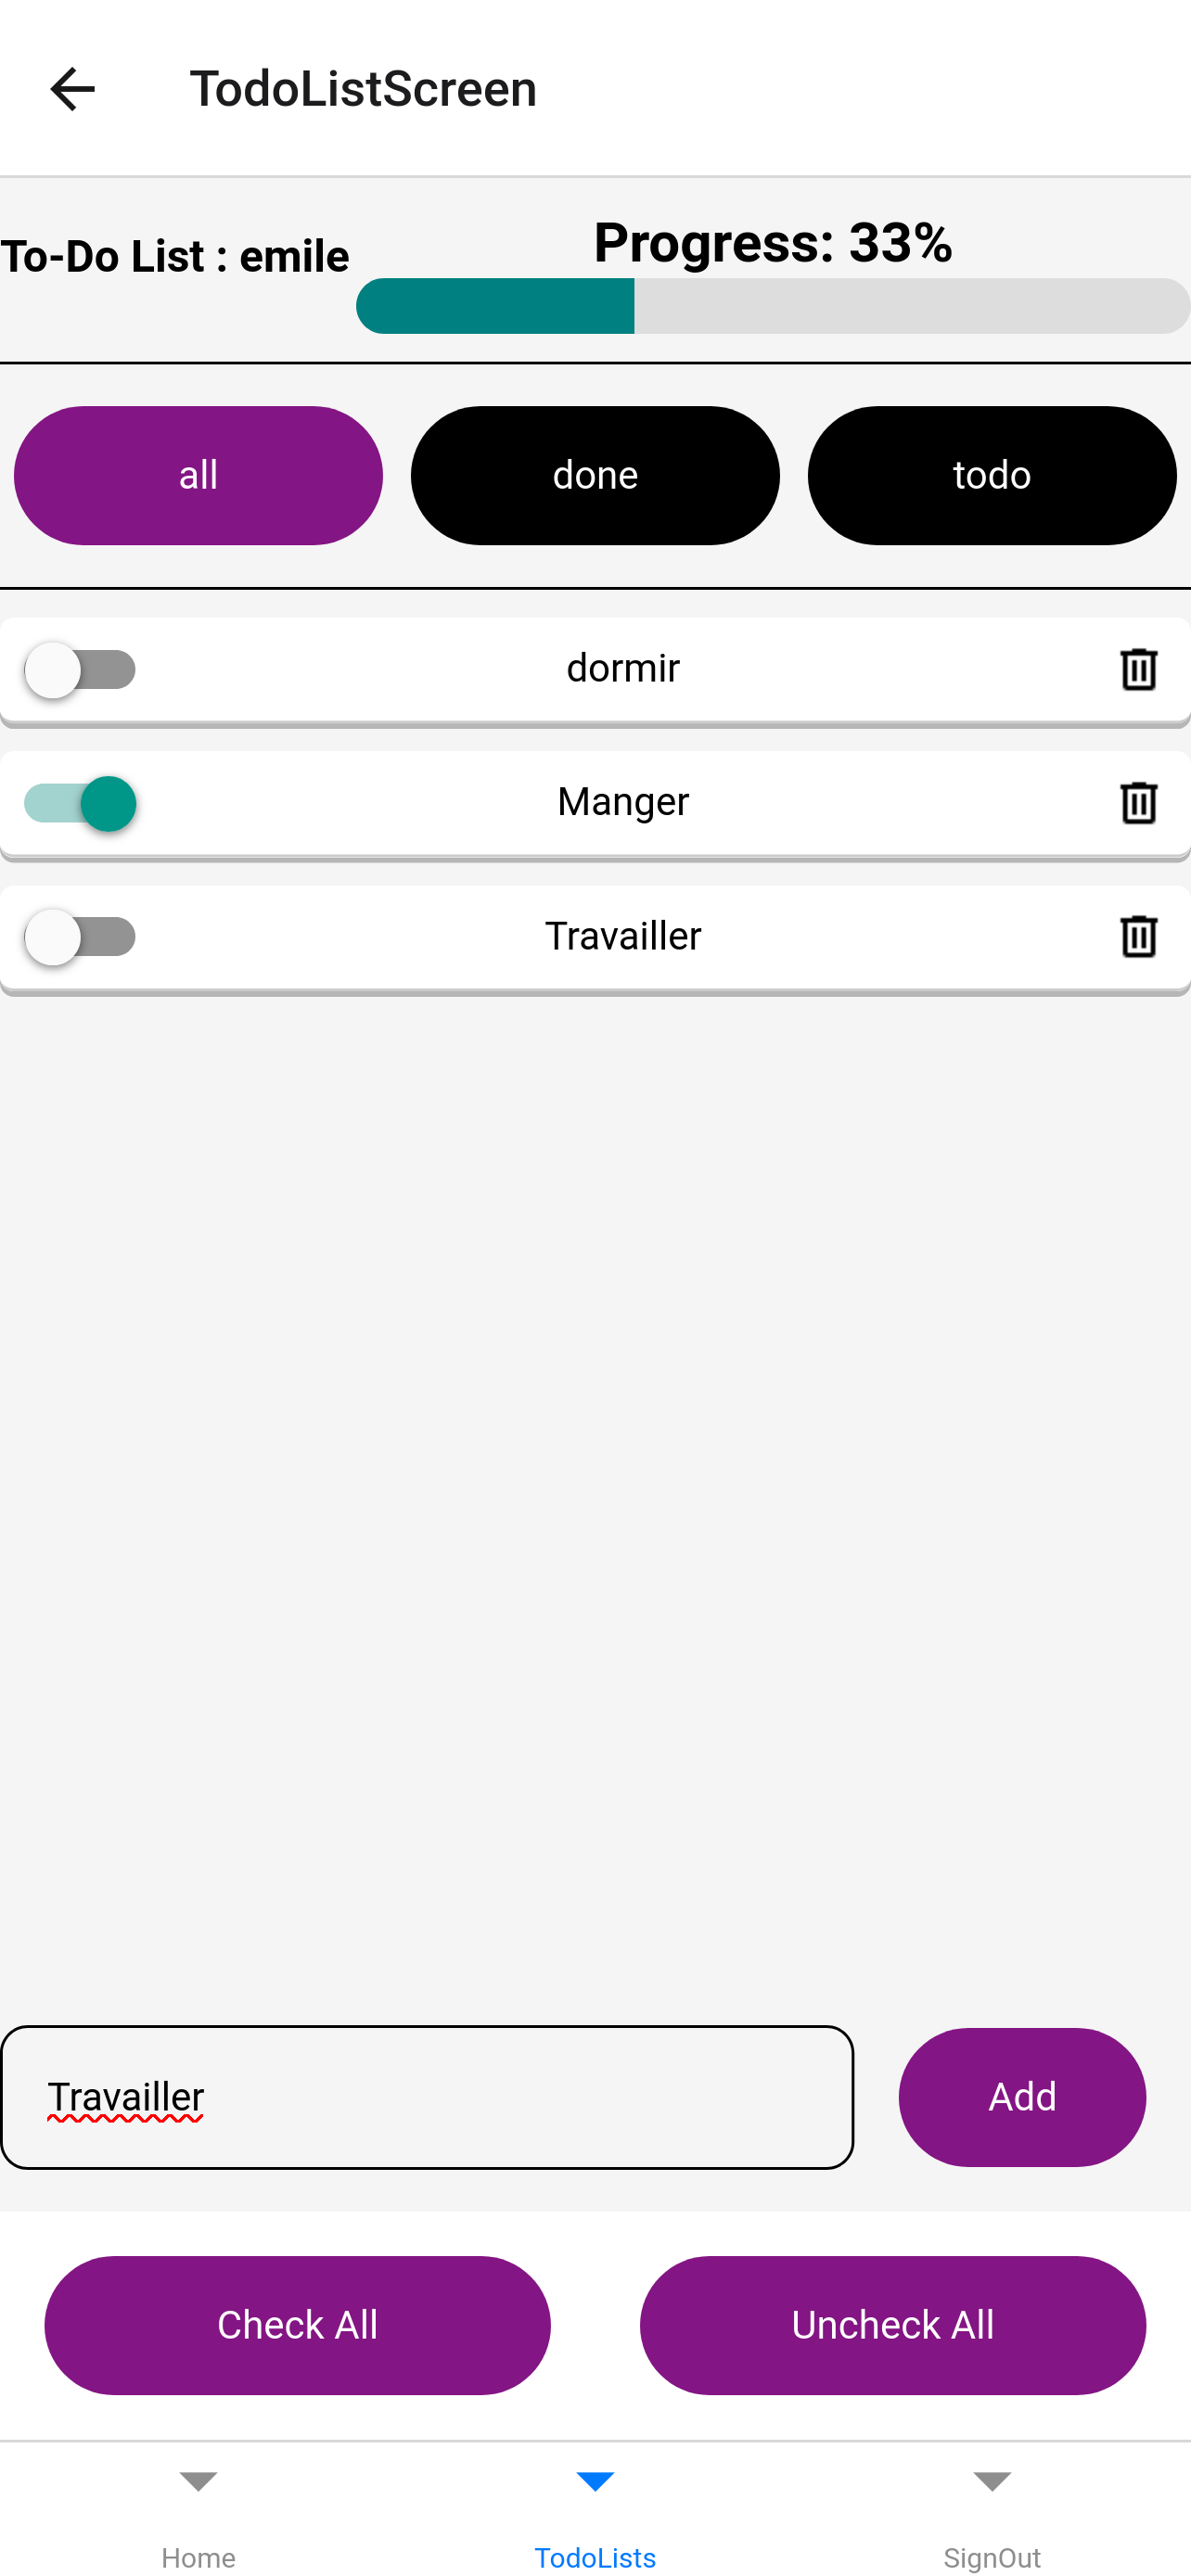
\includegraphics[width=0.4\textwidth]{images/tasks}
            \caption{Ecran de gestion des tâches}
            \label{fig:task}
        \end{figure}
        L'utilisateur peut créer une nouvelle tâche en cliquant sur le bouton \textbf{Nouvelle tâche} présent
        après avoir renseigné le nom de la tâche. Il peut également supprimer une tâche en cliquant sur la poubelle.
        Par défaut à la creation d'une tâche, elle est considérée comme non terminée. L'utilisateur peut la terminer
        en cliquant en sur le switch présent à droite de la tâche. Dans ce cas, la tâche est considérée comme terminée
        et est désormais grisé.\\
        Différents filtres sont disponibles pour afficher les tâches. L'utilisateur peut afficher;
        \begin{itemize}
            \item Les tâches non terminées
            \item Les tâches terminées
            \item Toutes les tâches
        \end{itemize}
        Il a aussi la possibilité de rendre toutes les tâches terminées (resp non terminées) en cliquant sur le bouton
        \textbf{Tout terminer} (resp \textbf{Tout non terminer}).

        \subsection{Autres écrans}{\label{subsec:other}}
        Nous avons aussi développé d'autres écrans comme l'écran de déconnexion, l'écran d'accueil.
        Ces écrans sont intermédiaires entre les écrans de gestion des listes de tâches et les écrans d'authentification.
            % Ajout des images des autres écrans

        \section{Développement de l'application}{\label{sec:dev}}
        Nous avons développé l'application à travers le framework \textbf{React native}. Ce framework permet de développer
        des applications mobiles multiplateformes. Il permet de développer des applications pour les plateformes
        \textbf{Android}, \textbf{IOS} et \textbf{Web}.\\
        Outre les composants natifs de React native, nous avons implémenté d'autres composants réutilisables. En effet,
        l'intérêt de React native est de pouvoir réutiliser des composants. Cela permet de rendre le code plus lisible
        et plus maintenable.\\





\end{document}